The Cypress CY7C68013C EZ-USB\textsuperscript{\textregistered} microcontroller on the RTSC provides a USB interface to the FPGA and provides JTAG programming capabilities without the need for separate JTAG programming hardware~\cite{DigilentNexys2rm}.  Unlike a general purpose microcontroller or FPGA, the Cypress microcontroller can connect directly to the USB signal lines with its integrated USB transceiver~\cite{CypressDS}.  Figure~\ref{fig:Cypress} shows the connections between the Cypress microcontroller and the FPGA on the RTSC.

%Table: USB Connector

%5V power supplied by the USB host at up to 500mA
%D+	Bidirectional asynchronous differential twisted pair serial data
%D-
%GND signal and power return

%The Cypress microcontroller acts a slave on the USB bus.  When the Nexys2 is connected to a PC, the Cypress microcontroller pulls the (check) high to signal the host that it is on the bus.

\begin{figure}[H]
	\centering 
		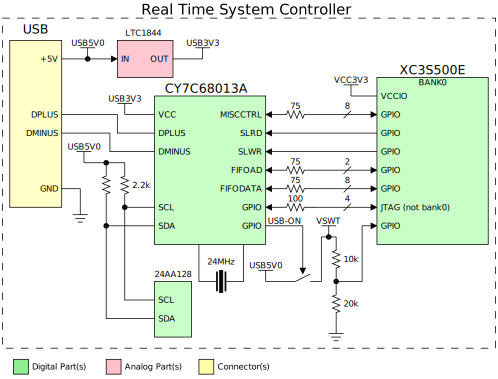
\includegraphics{./figures/Cypress} 
	\caption{Connections for the USB interface on the RTSC board~\cite{DigilentNexys2rm,DigilentNexys2sch}\label{fig:Cypress}}
\end{figure}

A USB peripheral must not draw more than 100mA from the host until it has negotiated the full power capabilities of the bus.  The Cypress microcontroller receives 3.3V power from a regulator connected directly to the 5V USB supply. The rest of the RTSC board can be powered from the USB supply, but if the entire RTSC board is to be powered by the USB supply voltage, it must not power all of its circuits immediately upon connection because the board would draw more than 100mA~\cite{DigilentNexys2rm}.  When the Cypress microcontroller has negotiated the full power capabilities of the bus, the USB-ON signal, which is connected to the gate of a NMOS transistor, is toggled connecting the USB5V0 voltage to the rest of the board~\cite{DigilentNexys2rm}.

Connections between the Cypress microcontroller have series resistors where the Cypress microcontroller signal can be an output.  This is to limit the current in the case of the FPGA pin being setup as an output simultaneously with the Cypress microcontroller.

Data transfer from the FPGA to the USB host is facilitated by a first in, first out (FIFO) buffer in the Cypress microcontroller.  A FIFO acts as a dual port memory allowing a device to push data into the memory; the FIFO will keep track of the memory address to be written.  The same device or a second device can then read from the memory and the FIFO will fetch the oldest data in memory that has yet to be read.  In this way, two devices, operating on different clocks or with other tasks to complete, can share data without being synchronized, or one device can store a stream of data and retrieve the data stream in the order written without the need for memory addressing logic.

Eight of the data connections between the Cypress microcontroller and the FPGA carry the FIFO data that can be written or read by the FPGA (FIFODATA).  The Cypress microcontroller internally reads or writes to the other side of the FIFO with data to or from the USB bus~\cite{CypressDS}.  A 24MHz crystal provides a dedicated clock to the Cypress microcontroller.  A 12pF capacitor is required from each terminal of the crystal to ground to stabilize the oscillation~\cite{DigilentNexys2rm}.  A 24AA128 EEPROM, that contains the Digilent\textsuperscript{\textregistered} firmware, is connected to the I$^2$C pins of the Cypress microcontroller, which are open-drain outputs and hysteresis inputs that must be pulled up to 3.3V even if unconnected~\cite{CypressDS}; although, the RTSC pulls these signals to USB5V0~\cite{DigilentNexys2sch}.
